%=================AVANCES Y PRUEBAS=================
% SENSORES DE PULSO

\section{Base de Datos}
Para poder realizar el desarrollo del proyecto se tiene que partir de un modelo de datos, mismo que será convertido en un modelo entidad relación. Para poder desarrollar la base de satos se tomaron en cuenta los siguientes puntos:

\begin{itemize}
	\item \textbf{Elaboración de maqueado de la app:} Se realizó la propuesta inicial del comportamiento de la aplicación por medio de interfaces, esto con base a los requerimientos especificados.
	
	\item \textbf{Abstacción de datos:} Se realizó un modelo de información con base en las necesidades identificadas en las interfaces
	
	\item \textbf{Modelado inicial de la Base de Datos:} Se realizó la propuesta inicial del modelo entidad relación para la base de datos.
	
	\item \textbf{Normalización de la Base de datos:} Se realizó la normalización de la base de datos hasta la tercer forma normal.
	
	\item \textbf{Generación de tablas de negocio:} Se generaron tablas en la base de datos para cubrir las necesidades especificas de negocio.
	
\end{itemize}

El modelado de la base de datos esta pensando en el negocio especifico para In-Help, haciendo uso de las buenas practicas en el modelado de negocios, esto con la única finalidad de poder tener un crecimiento con la afectación mínima a la BD.

\subsection{Maquetado de la App}
Para poder realizar el maquetado de interfaces de la aplicación se realizó el análisis correspondiente tomando como base los requerimientos funcionales definidos para el presente trabajo terminal. Una vez realizado el análisis pertinente se definieron los módulos con los que cuenta la aplicación mismos que se muestran en la figura \ref(fig:MaquetadoelaApp).

\begin{figure}[htbp!]
	\centering
	\fbox{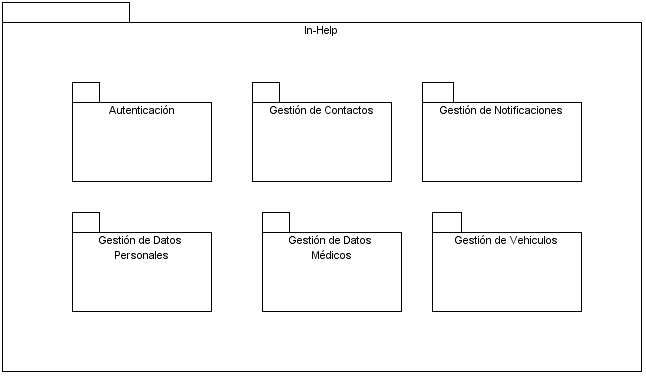
\includegraphics[width=0.9\textwidth]{AvancesPruebas/imagenes/Modulos_del_Sistema}}
	\caption{Módulos de la aplicación}
	\label{fig:MaquetadoelaApp}
\end{figure}

\subsection{Modelo Entidad Relación In-Help}

El modelo entidad relación de la aplicación se muestra en la figura \ref{fig:DB_InHelp}, mismo que se encuentra ordenado de forma correspondiente a los módulos con los que cuenta la aplicación para un mejor manejo de la misma.


\begin{figure}[htbp!]
	\centering
	\fbox{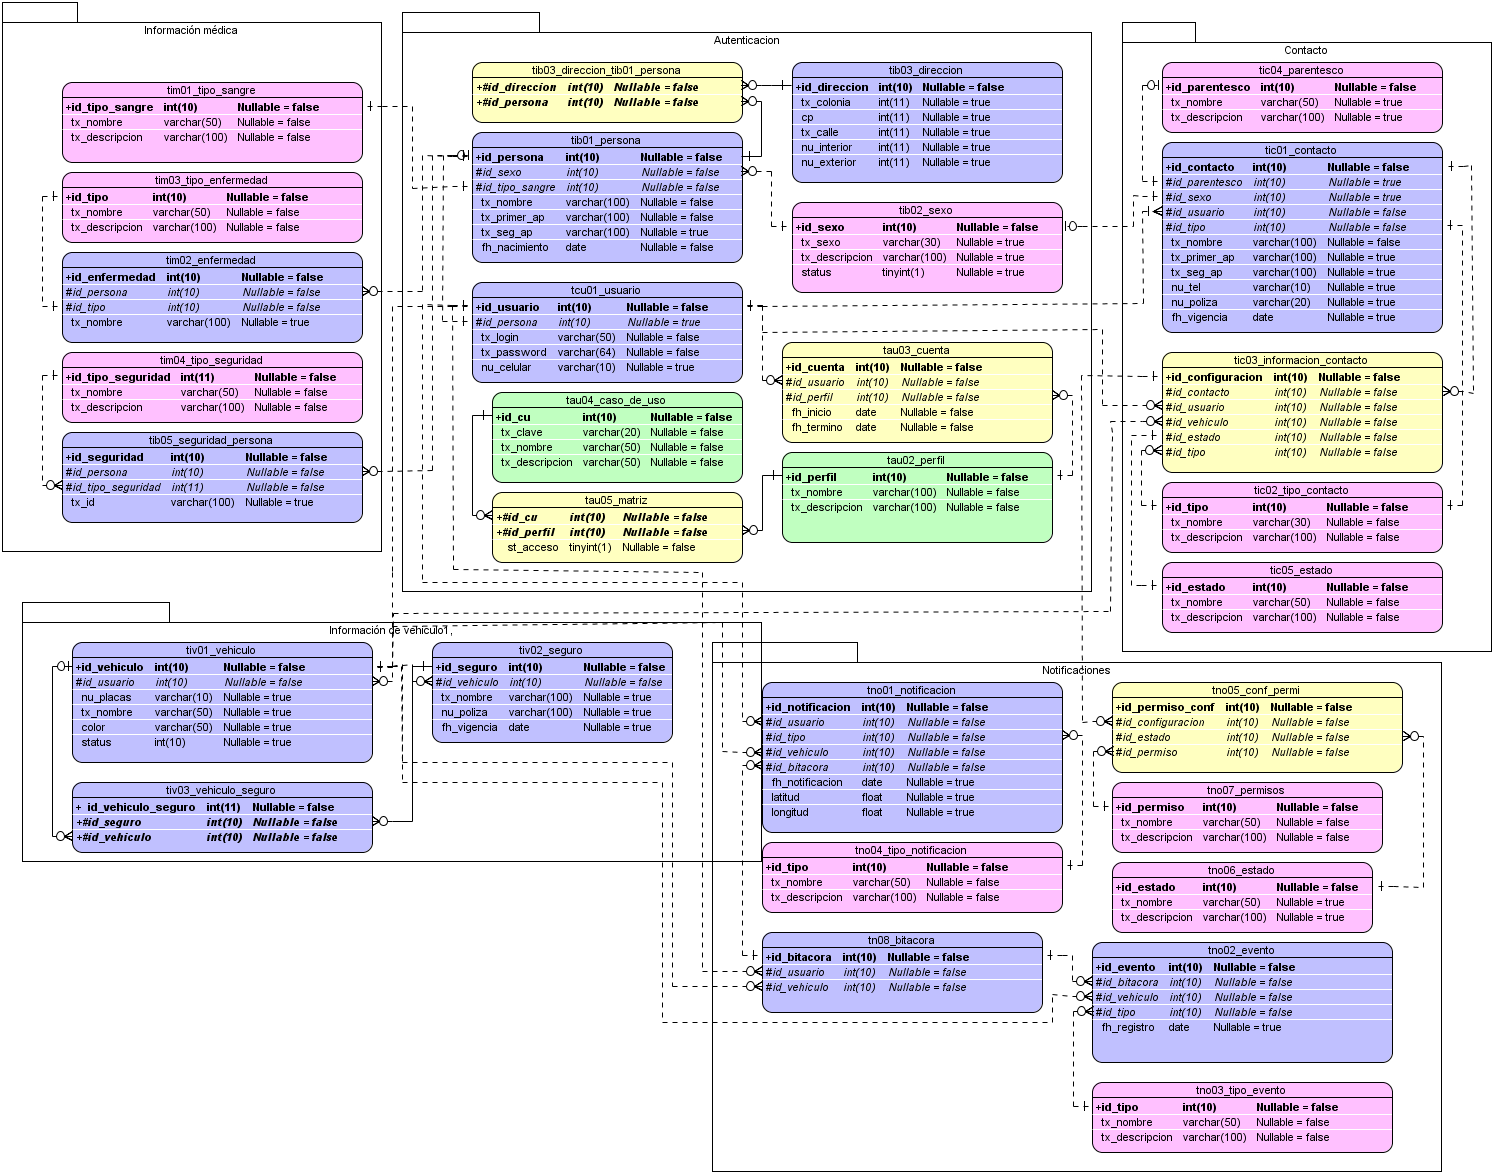
\includegraphics[width=0.9\textwidth]{AvancesPruebas/imagenes/DB_InHelp}}
	\caption{Modelo Entidad Relación In-Help}
	\label{fig:DB_InHelp}
\end{figure}

\subsection{Modelo Entidad Relación In-Help / Autenticación}
En la figura \ref{fig:BD_Autenticacion} se muestran las tablas correspondientes al módulo de autenticación el cual incluye casos de uso de registro de cuenta y de usuario, es esta la razón por la que se encuentra información de la persona, así como información propia de la cuenta.\\
De igual forma aquí se encuentran las tablas correspondientes a la matriz de acceso para un usuario, cabe mencionar que actualmente la aplicación existe un solo actor, el cual tiene acceso a todos los CU.\\
Las ventajas de manejar este tipo de modelos es una escalabilidad en la seguridad de la aplicación si es que así se requiere.
\begin{figure}[htbp!]
	\centering
	\fbox{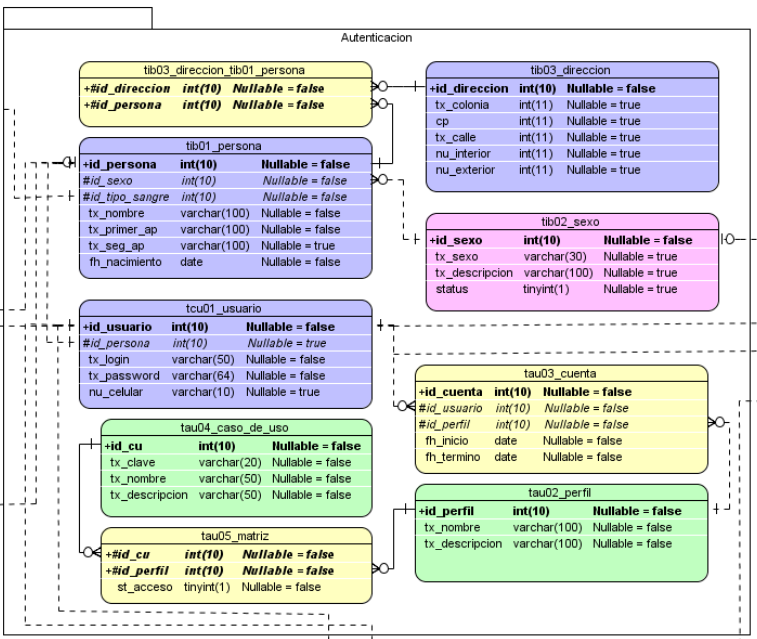
\includegraphics[width=0.9\textwidth]{AvancesPruebas/imagenes/BD_Autenticacion}}
	\caption{Autenticación}
	\label{fig:BD_Autenticacion}
\end{figure}

\subsection{Modelo Entidad Relación In-Help / Médica}
En la figura \ref{fig:BD_Medica} se muestran las tablas correspondientes al módulo de información médica, mismo que tiene dependencia directa con el modúlo de autenticación.
\begin{figure}[htbp!]
	\centering
	\fbox{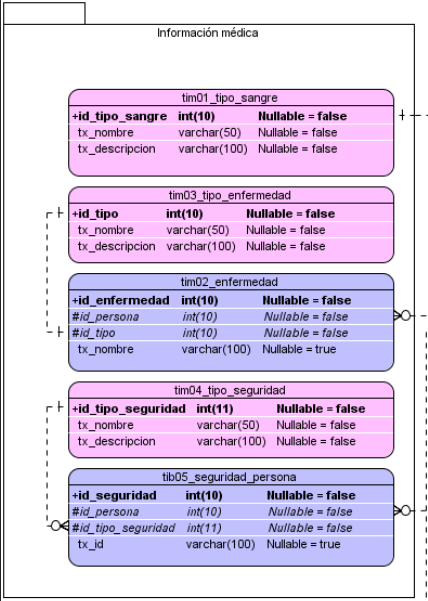
\includegraphics[width=0.9\textwidth]{AvancesPruebas/imagenes/BD_Medica}}
	\caption{Médica}
	\label{fig:BD_Medica}
\end{figure}
\subsection{Modelo Entidad Relación In-Help / Contactos}
\begin{figure}[htbp!]
	\centering
	\fbox{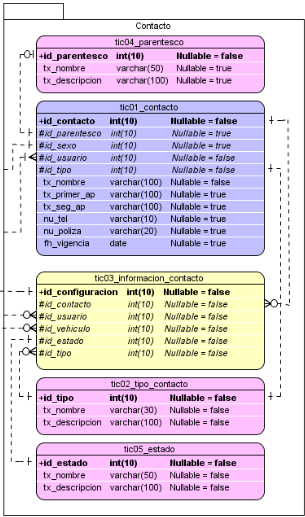
\includegraphics[width=0.7\textwidth]{AvancesPruebas/imagenes/BD_Contactos}}
	\caption{Contactos}
	\label{fig:BD_Contactos}
\end{figure}
\subsection{Modelo Entidad Relación In-Help / Vehiculos}
\begin{figure}[htbp!]
	\centering
	\fbox{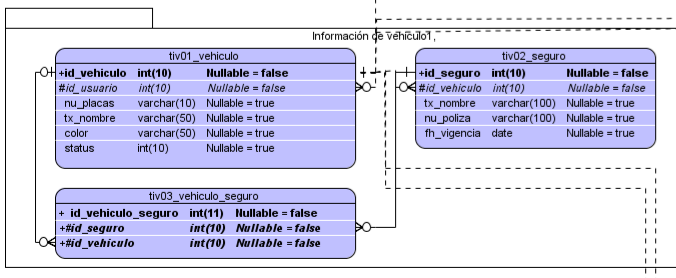
\includegraphics[width=0.9\textwidth]{AvancesPruebas/imagenes/BD_Vehiculo}}
	\caption{Vehículos}
	\label{fig:BD_Vehiculo}
\end{figure}
\subsection{Modelo Entidad Relación In-Help / Notificaciones}
\begin{figure}[htbp!]
	\centering
	\fbox{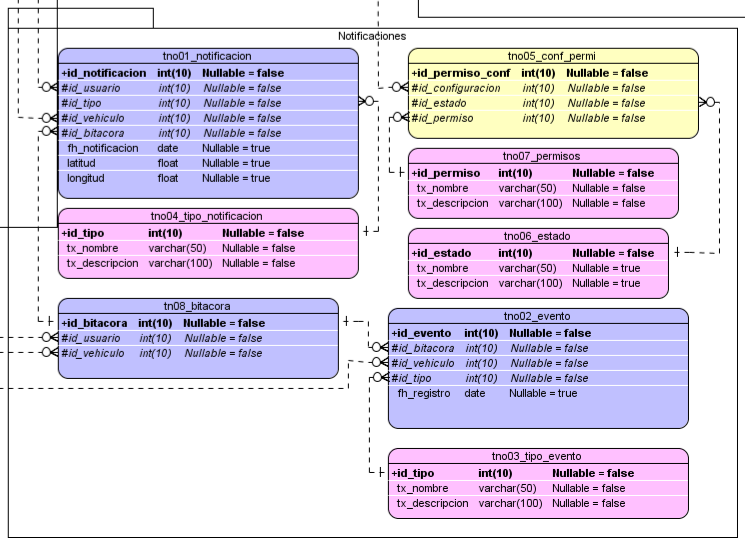
\includegraphics[width=0.9\textwidth]{AvancesPruebas/imagenes/BD_Notificacion}}
	\caption{Notificación}
	\label{fig:BD_Notificacion}
\end{figure}